\documentclass{beamer}
\usetheme{Madrid}
\usepackage[utf8]{inputenc}
\usepackage[czech]{babel}
\usepackage{times}

\title[Cloud computing] {Cloud computing}
\author[Autor: David Endrych] {David Endrych \\
 xendry02@stud.fit.vutbr.cz}
\institute[VUT BRNO] 
{
  Vysoké učení technické v Brně \\
  Fakulta informačních technologií
}
\date[ITY 2017] 
{}
\begin{document}
\frame{\titlepage}

\begin{frame}
    \frametitle{Co je to Cloud computing}
	\begin{block}{Definice}
	Cloud je obecný pojem pro cokoliv, kde jde o poskytování pronajímaných služeb přes Internet. 
	\end{block}
	\begin{block}{Význam slova cloud}
	Slovo cloud znamená anglicky mrak a pochází ze zvyku kreslit mrak ve schematických obrázcích komunikaci přes Internet.
	\end{block}
\end{frame}
\begin{frame}
\begin{center}
  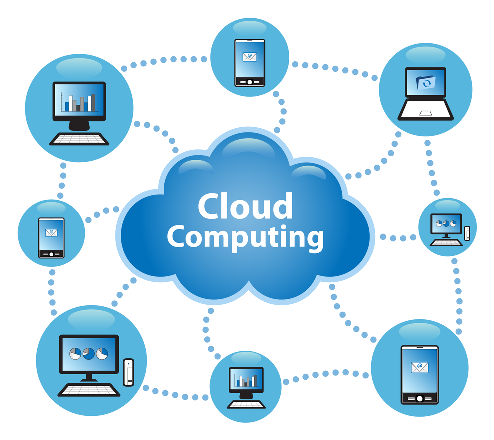
\includegraphics[scale=1]{scheme.eps}
\end{center}
\end{frame}
\begin{frame}
    \frametitle{Modely nasazení}
    \begin{itemize}
	\item \textbf{Veřejný -} Služba je poskytnuta široké veřejnosti 
	\item \textbf{Soukromý -} Cloud je provozován pro organizaci
	\item \textbf{Komunitní -} Infrastruktura cloudu je sdílena mezi organizacemi
	\item \textbf{Hybridní -} Kombinace veřejného a soukromého cloudu       
    \end{itemize}
\end{frame}
\begin{frame}
    \frametitle{Distribuční modely}
    \begin{itemize}
	\item \textbf{Saas -} Software jako služba   
	\item \textbf{Paas -} Platforma jako služba 
	\item \textbf{Iaas -} Infrastruktura jako služba
    \end{itemize}
\end{frame}
\begin{frame}
	\frametitle{Výhody}  
	\begin{itemize}
	\item Malé investice
	\item Možnost dynamicky měnit kapacitu
	\item Jednoduchost uživatelského rozhraní
	\item Rychlost nasazení
	\item SLA
	\end{itemize}
\end{frame}
\begin{frame}
	\frametitle{Nevýhody}
	\begin{itemize}
	\item Závislost na internetovém připojením
	\item Bezpečost
	\item Limitovaná nabídka softwaru a hardwaru poskytovatelem
	\item Může být pomalejší reakční doba
	\end{itemize}
\end{frame}
\begin{frame}
	\frametitle{Nejznámější poskytovatelé cloudových služeb}	
	\begin{figure}[h]
		
\includegraphics[scale=0.3]{amazon.eps}
		
\includegraphics[scale=0.12]{google.eps} \\
		
\includegraphics[scale=0.35]{ibm.eps}
		
\includegraphics[scale=0.12]{azure.eps}
	\end{figure}
\end{frame}
\begin{frame}
  \frametitle{Použité zdroje}    
  \begin{itemize}
   \item https://wiki.metacentrum.cz/wiki/Definice\_cloudu
   \item https://publi.cz/books/230/07.html
   \item https://cs.wikipedia.org/wiki/Cloud\_computing
  \end{itemize}
\end{frame}

\end{document}